\documentclass[12pt,letterpaper,titlepage]{article}
% Test comment added to lowryk local version - 3 May 2017

% LIST OF PACKAGES
\usepackage{setspace}
\usepackage{ragged2e}
\usepackage{graphicx}
\usepackage{times}              % Improve font over the default
\usepackage{amssymb,amsmath}		% Package for mathematical equations
\usepackage{color}
\usepackage{caption,booktabs,array}
\usepackage{microtype}          % Subtly improves word spacing
\usepackage{hyperref}
\usepackage{listings}			% Displays code lines (highly customizable)
\usepackage{marginnote}
%\usepackage{geometry}
\usepackage{pdfpages}
\usepackage[top=2.5cm, bottom=2.5cm, outer=5cm, inner=2.5cm, heightrounded, marginparwidth=4cm, marginparsep=.5cm]{geometry}

\definecolor{codegreen}{rgb}{0,0.6,0}
\definecolor{codegray}{rgb}{0.4,0.4,0.4}
\definecolor{codepurple}{rgb}{0.58,0,0.82}
\definecolor{backcolour}{rgb}{0.95,0.95,0.92}
\lstdefinestyle{mystyle}{
	backgroundcolor=\color{backcolour},
	commentstyle=\color{codegreen},
	keywordstyle=\color{magenta},
	numberstyle=\tiny\color{codegray},
	stringstyle=\color{codepurple},
	basicstyle=\small,
	basewidth=0.5em,
	breakatwhitespace=false,
	breaklines=true,
	captionpos=b,
	keepspaces=true,
	numbers=left,
	numbersep=5pt,
	showspaces=false,
	showstringspaces=false,
	showtabs=false,
	tabsize=1,
	aboveskip = 10pt,
	belowskip = 15pt
}
\lstset{style=mystyle}

% MACROS
% The FIXME macro
\newcommand{\fixme}[1]{\color{red}$<$\textbf{FIX ME: #1}$>$\color{black}}

% GLOSSARY
\usepackage[nonumberlist, nopostdot]{glossaries}
% Generate the glossary
\makeglossaries

%% APPENDIX MARGIN ENVIRONMENT
%\newenvironment{appendixgeometry}{%
%\geometry{top=2.5cm, bottom=2.5cm, outer=5cm, inner=2.5cm, heightrounded, marginparwidth=4cm, marginparsep=.5cm}}

% MAIN DOCUMENT
\begin{document}

	%Term definitions
\newglossaryentry{NI}{name=NI, description={Number of grid points in $i$-direction}}
\newglossaryentry{NJ}{name=NJ, description={Number of grid points in $j$-direction}}
\newglossaryentry{NK}{name=NK, description={Number of grid points in $k$-direction}}
\newglossaryentry{dtf}{name=dtf, description={Time step (non-dimensional)}}
\newglossaryentry{wsink}{name=wsink, description={Particle sinking velocity}}
\newglossaryentry{stress_top_x}{name=stress\_top\_x, description={Surface wind stress in x-direction}}
\newglossaryentry{stress_top_y}{name=stress\_top\_y, description={Surface wind stress in y-direction}}
\newglossaryentry{stress_top}{name=stress\_top, description={Surface wind stress magnitude}}
\newglossaryentry{wtotal}{name=wtotal, description={Total particle vertical velocity (advection + sinking)}}
\newglossaryentry{wzf}{name=wzf, description={Inverse thickness of a given $\sigma$-layer $\Delta \sigma /\Delta z = 1/\Delta z$} at cell faces}
\newglossaryentry{wz}{name=wz, description={Inverse thickness of a given $\sigma$-layer $\Delta \sigma /\Delta z = 1/\Delta z$} at cell center}
\newglossaryentry{D}{name=D, description={Model depth}}
\newglossaryentry{DL}{name=DL, description={Characteristic depth scale}}
\newglossaryentry{WL}{name=WL, description={Scaling coefficient for vertical velocity}}
\newglossaryentry{UL}{name=UL, description={Scaling coefficient for horizontal velocity}}
\newglossaryentry{EPS}{name=EPS, description={Rossby number}}
\newglossaryentry{zc}{name=zc, description={Depth of the cell centers (non-dimensional)}}
\newglossaryentry{zf}{name=zf, description={Depth of the cell faces (non-dimensional)}}
\newglossaryentry{pfac}{name=pfac, description={Stretching coefficient used ot determine vertical grid spacing}}
\newglossaryentry{dztop}{name=dztop, description={Thickness of the uppermost cell (non-dimensional)}}
\newglossaryentry{$u$}{name=u, description={Velocity in $x$-direction (non-dimensional)}}
\newglossaryentry{$v$}{name=v, description={Velocity in $y$-direction (non-dimensional)}}
\newglossaryentry{$w$}{name=w, description={Velocity in $z$-direction (non-dimensional)}}
\newglossaryentry{dx}{name=dx, description={Grid-spacing in the $x$-direction (in m)}}
\newglossaryentry{dy}{name=dy, description={Grid-spacing in the $y$-direction (in m)}}




	\title{User Manual for PSOM\\[.5cm] 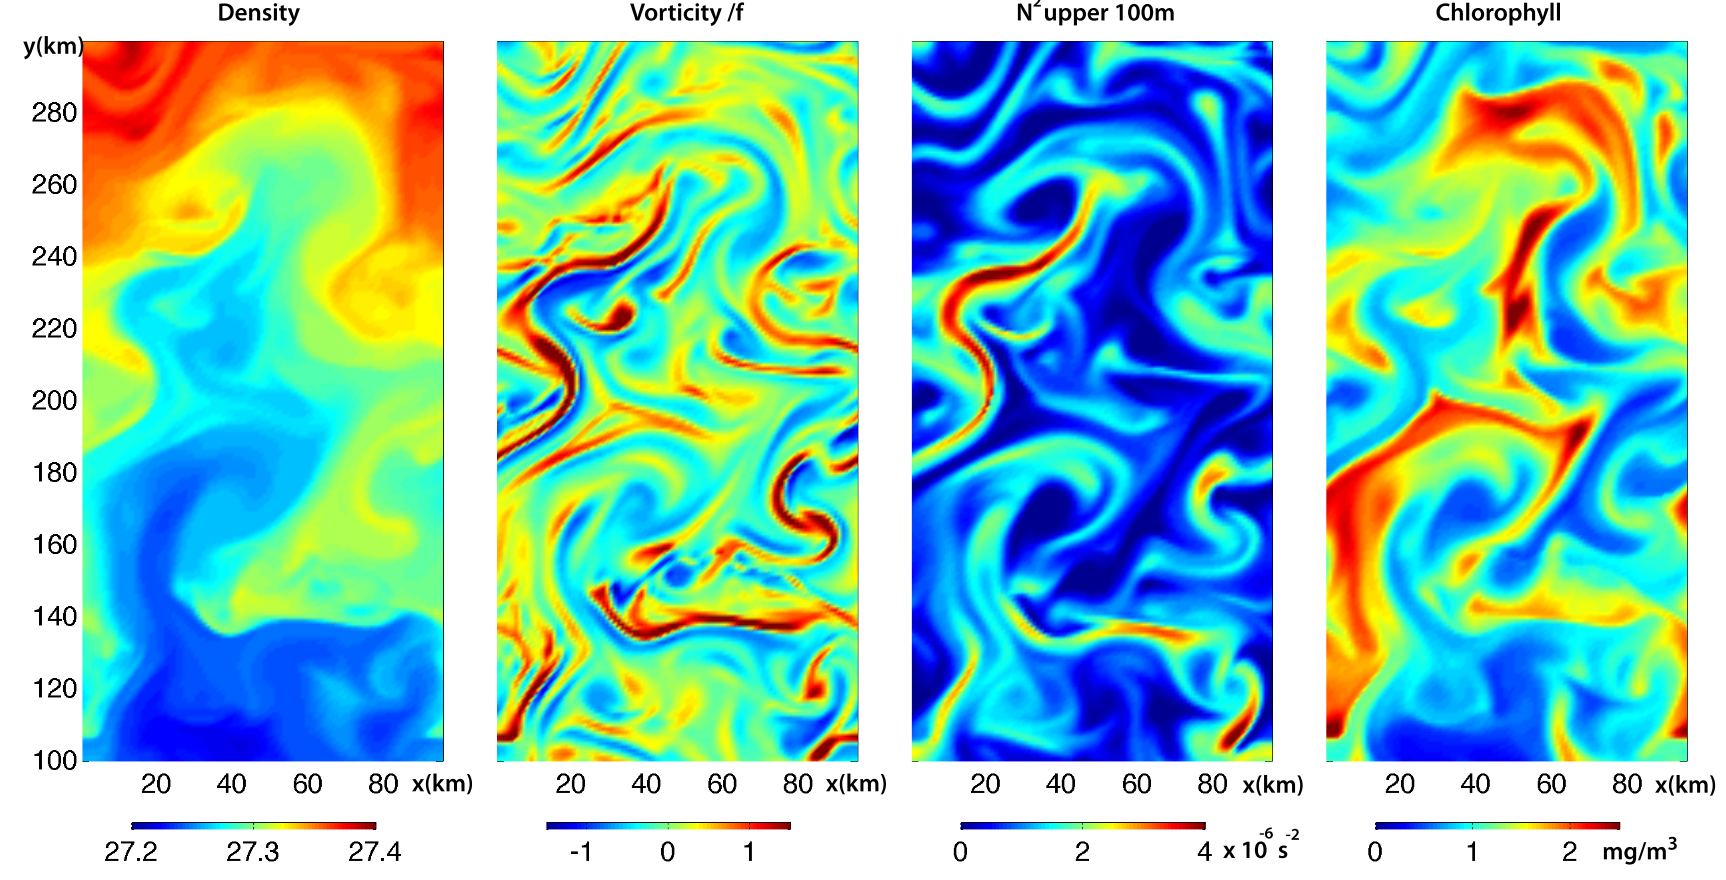
\includegraphics[width =\linewidth]{PSOM_cover_photo}}
	\author{Ocean and Environmental Processes\\ Dr. Amala Mahadevan's Lab\\ {\small Compiled by M. Dever}}
	\date{\today}
	\maketitle

\tableofcontents
\pagebreak

\section{Introduction}


%FROM README FILE :

%* GENERAL DESCRIPTION

PSOM, pronounced "soam" (the nectar derived from the churning of the oceans in Indian mythology), stands for Process Study Ocean Model.
It is a versatile, three-dimensional, non-hydrostatic, computational fluid dynamical model for oceanographic (as well as other) applications (Mahadevan et al., 1996a,b).
The model uses the finite volume method on a structured grid with boundary fitted coordinates (topography conforming sigma grid in the vertical, and boundary conforming in the horizontal).
The model has a free-surface. It can be used for large- and small-scale phenomena and can be run in hydrostatic or non-hydrostatic mode (Mahadevan, 2006). It uses a highly efficient solution procedure that exploits the skewness arising from the small geometrical aspect (depth to length scale) ratio of the ocean to speed up the solution of the non-hydrostatic pressure, which is solved by the multigrid method.

The model has been used for a number of process studies, including investigation of the vertical transport of nutrients for phytoplankton production (Mahadevan and Archer, 2000) and the dynamics of submesoscale processes (Mahadevan and Tandon, 2006; Mahadevan, Tandon and Ferrari, 2010). Since the non-hydrostatic model is well-posed with open boundaries, it can be used as a nested high-resolution model with time-varying boundary conditions applied from a coarser resolution general circulation model (Mahadevan and Archer, 1998). The model is thus ideally suited for high-resolution, limited-region modeling studies.


\section{Downloading PSOM}

\begin{enumerate}
\item Download the latest version of PSOM from GitHub. Users are strongly encouraged to track the modifications and improvements made to PSOM, and to submit them for review through GitHub.
\item Unzip the file into a directory (e.g., \texttt{V1.0-master})
\item Go to the "\texttt{V1.0-master/code}" directory and follow the instructions detailed below.
\end{enumerate}

\begin{itemize}
	\item[\textbf{NOTE}]: Hereafter, filepaths are always specified with respect to the directory\\ "\texttt{V1.0-master/code}".
\end{itemize}


\section{Setting-up PSOM}

\subsection{Fortran compiler and bash$\_$profile}

Before setting-up PSOM, it is important to make sure that the compiler that will be used to compile PSOM is properly installed. Once the compiler is properly installed, the file \texttt{.bash$\_$profile} should be edited to include the proper paths. In the example below, the \texttt{.bash\_profile} includes 3 different paths where the compiler could be located (\textsl{/opt/intel/composer$\_$xe$\_$2015/bin}, \textsl{/usr/local}, and \textsl{/opt/intel/bin})
.
\begin{lstlisting}[language=sh, breaklines]
#bash_profile

# PSOM environment variables
export DYLD_LIBRARY_PATH=/opt/intel/lib
export PATH=$PATH\:/opt/intel/composer_xe_2015/bin:/usr/local:/opt/intel/bin

\end{lstlisting}

\subsection{\texttt{optfile} and \texttt{configure.sh}}

Before being able to compile PSOM, a few necessary steps must be taken:

\begin{itemize}
	\item[\textbf{Step 1:}] \textbf{Update the \texttt{optfile}}\\
	Edit the line "\textit{fcomp=...}" to specify the proper compiler (e.g., ifort, pgf95, etc.). If compiler is modified, the user is encouraged to scan through the ./optfile to make other necessary modifications (e.g., activation of gotm library, define\_parallel flag, etc.).

	\item[\textbf{Step 2:}] \textbf{Run \texttt{configure.sh}}
\begin{lstlisting}[language=sh, breaklines]
		sh tools/configure.sh
\end{lstlisting}
Running \texttt{configure.sh} will search for makedepend (which is necessary to create the makefile). The script will stop if makedepend is not installed. The makefile file will only be created if makedepend can be called. Therefore, the user should download makedepend, which is free and widely accessible. For instance, on mac, you can simply type (if you have macport installed):
\begin{lstlisting}[language=sh, breaklines]
 sudo port install makedepend
\end{lstlisting}
A conda environment to configure, compile, and run PSOM on the WHOI HPC (Poseidon) is included as `environment$\_$compile.yml'

If you chose to use netcdf, an attempt to use nc-config will be tried. If nc-config is present, it will be used in order to set the links to netcdf libraries appropriately; If not, you can complete this step yourself by linking the executable to the netcdf libraries. To do so, edit ./optfile before going to the next step.

To summarize, This step has 2 effects: (1) modify \texttt{optfile}, and (2) customize \texttt{namelist}. Failures in running \texttt{configure.sh} can likely be avoided by correctly installing makedepend and/or netcdf libraries.

\end{itemize}

\section{Running PSOM}
\label{sec: cleanconmpilerun}
After properly setting-up PSOM, you can simply follow the "clean, compile, run" sequence:

\begin{itemize}
	\item[\textbf{clean:}] This step is only necessary if a new experiment is compiled. If re-compiling the same experiment, there is no need to run \texttt{clean.sh}. \texttt{clean.sh} is ran using:
\begin{lstlisting}[language=sh, breaklines]
	sh tools/clean.sh
\end{lstlisting}

	\item[\textbf{compile:}] Running \texttt{compile.sh} will (1) create the makefile in the folder mkfile, and (2) compile the fortran code. A failure during step 4 most likely indicates that there is an error in the fortran code. \texttt{compile.sh} is ran using:
\begin{lstlisting}[language=sh, breaklines]
	# To compile PSOM using default setup (cf. superceding trick)
	sh tools/compile.sh

	# To compile a specific experiment, such as the wiggle test case
	sh tools/compile.sh wiggle
\end{lstlisting}
		\item[\textbf{run:}] Runs the executable generated by the compiling step. It uses the \texttt{namelist} file to define the experiment's parameters (e.g., time step, output path, etc.; see Section \ref{sec: namelist}).
\begin{lstlisting}[language=sh, breaklines]
	# To run the wiggle experiment
	/exe/nh_wiggle < wiggle/namelist_wiggle
\end{lstlisting}
\end{itemize}

\section{Test Cases}
\subsection{Wiggles}
\label{sec: Wiggles}
\begin{lstlisting}
- wiggle      : This is a testcase with a wiggling front over a flat topography.
\end{lstlisting}

\subsection{NA}
\label{sec: NA}
\begin{lstlisting}
- NA          : This is a much more complex simulation of three fronts that go unstable. This casse has particles and tracers for biology.
\end{lstlisting}

\subsection{Shelfbreak}
\label{sec: Shelfbreak}
\begin{lstlisting}
- shelfbreak  : Simulation of the Middle Atlantic Bight shelfbreak with a shelf front and a shelfbreak font. The topography includes a sharp slope at the break. It shows how to use the "user" namelist.
\end{lstlisting}

\subsection{NP\_summer and NP\_winter}
\marginnote{\vspace{-.5cm} \raggedright \small \textbf{\underline{North Pacific Experiment}}\\Simulation developed by M. Dever as part of the NASA-funded Pre-ExPORTS project.}
This model experiments aims at capturing the ocean condition in the northeast Pacific, centered on Ocean Station Papa OSP (\url{https://www.pmel.noaa.gov/ocs/Papa}), in both the winter and summer time. Simulations' details can be found in Dever et al. (in review) \footnote{[submitted] Dever M., Nicholson D., Mahadevan A. Size-differentiated Export in different Dynamical Regimes in the Ocean. Submitted to Global Biogeochemical Cycles}. It relies on three fronts in a channel zonal configuration, with both heat and wind forcing.

\section{Setting up your PSOM simulation}
\subsection{Create your experiment directory}
\marginnote{\raggedright \small \textbf{\underline{Superseding trick}}\\When compiling, priority is given to the routines present in the experiment folder, over the source code present in \texttt{model/src/}. For example, if the wiggle experiment is compiled, any routines located in \texttt{wiggle/src/} will be used over the matching routines located in \texttt{model/src/}.}

For every experiment you want to conduct, create a directory that will contain the source files specific to this experiment. As an example, let's say you want to create an experiment named "my\_experiment". First, create a directory \texttt{my\_experiment/}, in which you will create two subdirectories \texttt{my\_experiment/inc} and \\\texttt{my\_experiment/src} . You can either create these directories manually, or you can run:

\begin{lstlisting}[language=sh]
# Copies the template directory
cp -r expe_template my_experiment
\end{lstlisting}
Whether you are a user or a developer, \textbf{you are strongly invited to leave untouched the files contained in \texttt{model/}}. This directory is designed to contain the latest version of the model, which is common to every user at a given time. For every routine that will be specific to \texttt{my\_experiment}, a new subroutine should be created in \texttt{my\_experiment/src/}. This can be achieved using the following command:
\begin{lstlisting}[language=sh]
# Copies the initial conditions subroutine
cp model/src/ini_st.f90 my_experiment/src
\end{lstlisting}
The compiling step (see Section \ref{sec: cleanconmpilerun}) includes a superseding procedure that will take into account the new version of \texttt{ini\_st.f90} (in \texttt{my\_experiment/src/}) and disregard the standard version found in \texttt{model/src/}. More precisely, it will create the makefile based on this new state of the model (in \texttt{./mkfile}), compile and create the executable \texttt{exe/nh\_my\_experiment}. More details on \texttt{compile.sh} may be found by running:

\begin{lstlisting}[language=sh]
# Provides more information on compile.sh
sh tools/compile.sh -help
\end{lstlisting}

\subsection{Defining your model grid}

The grid size is defined in \texttt{size.h}. If you wish to modify the grid size, you must first copy \texttt{size.h} into your experiment's directory:

\begin{lstlisting}[language=sh]
# Copies the grid file
cp model/inc/size.h my_experiment/inc
\end{lstlisting}

Grids used in previous experiments are listed in this file and commented out. If your grid appears in a commented line, Comment the uncommented line and uncomment the one you want. Be aware that if your grid set requires more than 2Go, you might experience compilation issues. If so, you may fix the issue by editing \texttt{tools/genmakefilel} to replace the default compiling options by:

\begin{lstlisting}[	basicstyle=\footnotesize, numbers=none]
 fflags_o="-fpp -real-size 64 -mcmodel medium -shared-intel -stand 03 -u"
 fflags_e="-fpp -real-size 64 -mcmodel medium -shared-intel -stand 03 -u"
\end{lstlisting}

If your grid set does not appear in \texttt{my\_experiment/inc/size.h}, you can create the required line. Defining the model grid is not straight-forward, because of the multi-grid solver mgrid \fixme{(See Section)}. The multi-grid solver is used to allow the reuse of array space in \texttt{mgrid.f90} \fixme{insert link to function?}. Although this issue could now be circumvented by making use of f90's dynamic allocation of memory, the code was originally in fortran77, explaining the need for space re-allocation. A step-by-step approach to defining your own grid is provided below:

\begin{enumerate}
	\item Choose grid dimensions $NI$, $NJ$, and $NK$ (i.e., the number of grid cells in $x$, $y$, and $z$ directions) such that the grid can be subdivided a maximum number of times by a factor of 2 to form "$ngrid$" levels of grid. For example, choosing $NI=48$, $NJ=24$, and $NK=32$ constrains the grid levels to 4 (i.e., $ngrid = 4$), because:

	\begin{align*}
		NI:& \; 48; 24; 12; 6; 3 &\text{(5 grid levels)}\\
		NJ:& \; 24; 12; 6; 3 &\text{(4 grid levels)}\\
		NK:& \; 32; 16; 8; 4; 2 &\text{(5 grid levels)}\\
	\end{align*}
	The number of grid points possible for a specific $ngrid$ can be computed by multiplying prime numbers (2, 3, 5, 7, etc.) by $2^{ngrid-1}$. Table \ref{tab: ngrid} lists some of the most commonly used number of grid points, depending on the number of grid levels $ngrid$.

	\item Compile \texttt{tools/preproc.f90}:
\begin{lstlisting}[language=sh]
# Compiles preproc.f90 (e.g., using ifort)
ifort preproc.f90 -o preproc
\end{lstlisting}

	\item Runs \texttt{preproc.f90} and fill the values that are asked:
\begin{lstlisting}[language=sh]
# Runs preproc
./preproc
\end{lstlisting}

\item Copy/Paste the last line the program provides in \texttt{my\_experiment/inc/size.h}. Below is an example for $NI=96$, $NJ=160$, and $NK=32$ (hence $ngrid=5$, see Table \ref{tab: ngrid}):
\begin{lstlisting}[	basewidth=0.5em]
./preproc
	number of grid levels in mgrid, ngrid =
5
	input the grid info
	NI =
96
	NJ =
160
	NK =
32
	Number of grid points on fine grid: nx,ny,nz   96   160   32
m,ntint,ntout,nbc(m) 1      491520      539784       47104
m,ntint,ntout,nbc(m) 2       61440       73800       11776
m,ntint,ntout,nbc(m) 3        7680       10920        2944
m,ntint,ntout,nbc(m) 4         960        1848         736
m,ntint,ntout,nbc(m) 5         120         384         184
Copy the following line to size.h
INTEGER, PARAMETER :: NI=96, NJ=160, NK = 32, ngrid=5, maxout=626736, maxint=561720, int1=491520
\end{lstlisting}
\end{enumerate}

\begin{table}[t]
	\caption{\label{tab: ngrid} Number of grid points associated with a specific number of grid levels $ngrid$. These numbers can be computed by multiplying prime numbers (2, 3, 5, 7, etc.) by $2^{ngrid-1}$. Each experiment's number of grid levels is set by the minimum $ngrid$ associated with $NI$, $NJ$, and $NK$.}
	\centering
	\begin{tabular}{ccrrrrrrrr}
		\toprule
		$ngrid$& & \multicolumn{8}{c}{Number of grid points ($NI$, $NJ$, or $NK$)}\\
		\midrule
		4 & &  16  &  24  &  40  &  56  &  88  &  104  &  136  &  152 \\
		5 & &  32  &  48  &  80  &  112  &  176  &  208  &  272  &  304 \\
		6 & &  64  &  96  &  160  &  224  &  352  &  416  &  544  &  608 \\
		7 & &  128  &  192  &  320  &  448  &  704  &  832  &  1088  &  1216 \\
		\bottomrule
	\end{tabular}
	\label{tab: multiple_regression}
\end{table}

\subsection{cppdefs.h}
\label{sec: cppdefs}
This file defines the different options to be used in the experiment. Again, it is recommended to copy this file into the experiment folder (e.g., \texttt{my\_experiment/inc/} before making any modifications. To include (exclude) an option, use \#define (\#undef) $option\_name$. The file includes 13 options:

\begin{enumerate}
	\item[$runtracmass$ :] placeholder
	\item[$periodic\_ew$ :] placeholder
	\item[$periodic\_ns$ :] placeholder
	\item[$allow\_particle$ :] If defined, allows the seeding of particles in the experiment. Please refer to section \fixme{ref to particle section} for a detailed explanation on particle seeding.
	\item[$rhoonly$ :] If defined, only the density field $rho$ is used. The density field is stored in the salinity array ($s$; see \texttt{evalrho\_rho.f90}). If not defined, $rho$ is computed from the salinity ($s$) and temperature ($T$) fields (see \texttt{evalrho\_sT.f90}).
	\item[$relaxation$ :] placeholder
	\item[$fixed\_bottom\_thickness$ :] placeholder
	\item[$file\_output$ :] placeholder
	\item[$file\_output\_cdf$ :] placeholder
	\item[$file\_output\_bin$ :] placeholder
	\item[$gotm\_call$ :] placeholder
	\item[$implicit$ :] placeholder
	\item[$parallel$ :] placeholder
\end{enumerate}


\subsection{namelist}
\label{sec: namelist}
This file defines key parameters relating to the experiment (e.g., grid resolution, time step, diffusion, output, ...). Again, it is recommended to copy this file into the experiment folder (e.g., \texttt{my\_experiment/} before making any modifications. Each parameter in the file is either self-explanatory or include a short description as a comment.

<<<<<<< Updated upstream
\subsection{Defining the initial conditions}
Initial conditions can be specified either in the corresponding subroutines, or from an input file. The former approach is used in the Shelfbreak test-case (see Section \ref{sec: Shelfbreak}), where the temperature and salinity distributions are determined from analytical expressions in DO-loops, and only requires a limited knowledge of the model grid. The latter approach can sometimes be more practical, especially when using available data products to initialize the model. However, this approach requires mapping the data used to initialize the experiment to the pre-defined model grid.

The horizontal grid is relatively straightforward to determine, given the grid size specified in \texttt{my\_experiment/inc/size.h} (i.e., $NI$ and $NJ$), and the grid resolution specified in \texttt{my\_experiment/namelist} (i.e., $dx$ and $dy$). The location of each grid point can be computed using the following equations:
\begin{align}
x(i) &= -dx/2 + i dx; &i &= (0, 1 , 2 \ldots NI, NI+1)\\
y(j) &= -dy/2 + j dy; &j &= (0, 1 , 2 \ldots NJ, NJ+1)
\end{align}

The initial conditions in the temperature and salinity: Talk abour the rhoonly flag, the way to set initial conditions, etc...

<<<<<<< Updated upstream
\subsection{Wind stress}
To specify a customized wind forcing, the code in \texttt{wind\_stress.f90} can be modified. The wind stress at the surface is prescribed to the model through the variables $stress\_top\_x$, $stress\_top\_y$, and $stress\_top$. The dimensions of these three variables are ($NI$,$NJ$) (see \texttt{header.f90}). The surface wind stress can be read from a file:

\begin{lstlisting}[	basewidth=0.5em, language=fortran]
! Import the wind stress time series for model forcing
if (step.eq.1) then
		open(unit=17, file='youfilefullpath.in')
		do i=1,nsteps
				read(17,fmt="(F5.10,F5.10)") stressxTS(i),stressyTS(i)
		end do
		close (17)
		PRINT*,"Read wind stress"
end if
stress_top_x = stressxTS(step)
stress_top_y = stressyTS(step)
\end{lstlisting}
or specified as a constant:

\begin{lstlisting}[	basewidth=0.5em, language=fortran]
stress_top_x = 0.05d0
stress_top_y = 0.01d0
PRINT*,"Read Wind Stress"
\end{lstlisting}

If your domain includes solid boundary (i.e., no periodicity), it is recommended to damp the surface wind stress close to the boundaries, to avoid upwelling/downwelling. Below is an example of wind stress damping at the north/south boundaries using a tanh profile. A similar approach can be used in the east/west direction.

\begin{lstlisting}[	basewidth=0.5em, language=fortran]
! Apply a tanh profile in the meridional direction
ycenter = 0.5*(yc(NJ)+yc(1))	! Find the middle of the domain
ywindmin = 10.0 							! Starts damping 10 km from southern boundary
ywindmax = yc(NJ)-10.d0   	   ! Starts damping 10 km from northern boundary
edge = 0.06    							! tightnness of the padding in the wind stress

do j=1,NJ
		if (yc(j).lt.yc(NJ/2)) then
				stressprofile(j) = 0.5*(tanh(edge*(yc(j)-ywindmin)*PI)+1.d0)
		else
				stressprofile(j) = -0.5*(tanh(edge*(yc(j)-ywindmax)*PI)-1.d0)
		end if
end do

do j=1,NJ
		do i=1,NI
				stress_top_x(i,j) = stressxTS(step)*stressprofile(j)
				stress_top_y(i,j) = stressyTS(step)*stressprofile(j)
		end do
end do
\end{lstlisting}

\subsection{Surface Heat Fluxes}

\section{Particle tracking in PSOM}
PSOM offers the option to release and track particles "online" (i.e., as part of the numerical simulation). To activate this option, the allow\_particle options must be defined in \texttt{inc/cppdefs.h} by including (See Section \ref{sec: cppdefs}):
\begin{lstlisting}[	basicstyle=\footnotesize, numbers=none]
#define allow_particle
\end{lstlisting}
The particle tracking code has been written for a rectangular grid only, and cannot be used ``as is" for a non-rectangular model grid.
\subsection{Non-sinking particles}
While key particle parameters are set in \texttt{namelist} (e.g., particle number, frequency of outputs, etc.; see Section \ref{sec: myparticletracking}), the seeding and advection of particles is controlled by the code included in \texttt{particles.f90}. The file includes the following subroutines:

\begin{itemize}

	\item[\textit{open\_ parti\_ files}:] This subroutine creates the output files where the particle characteristics will be saved. The number of output files is specified in \texttt{namelist} and must be a factor of the total number of particles ($NPR$). Increasing the number of output files reduced the size of the individual files, which proves to be useful when dealing with a very large number of particles. The output files are unformatted binary files.

	\item[\textit{save\_ parti}:] This subroutine loops through all the particles and writes the specified variables. The number of variables saved is important, as it must be known to read the unformatted binary output files.

	\item[\textit{ini\_ particles}:] This subroutine is called when the model timestep matches the particle initialization timestep specified in \texttt{namelist}. This is where the seeding of particle is defined. By default, all particles are released below the surface layer in the middle of the model domain. To personalize the release of particles, see Section \ref{sec: perso_particles}.

	\item[\textit{get\_ parti\_ vel}:] This subroutine interpolates the physical model's velocity field onto the particles' positions (using \textit{interp\_trilinear}; see below). The \textit{get\_parti\_vel} subroutine also interpolates variables of interest onto the particles position (e.g., salinity, temperature, density, vorticity, etc.).

	\item[\textit{parti\_ forward}:] This subroutine extrapolates the position of a particle at the next timestep t+1 using a 2$^{nd}$ order Adams-Bashforth scheme. As an example, the position of the particle in the zonal direction is computed using:

	\begin{equation*}
		(i,j,k)_{t+1}= (i,j,k)_{t} + dtf \times \frac{1}{2}[3(u,v,w)_{t+1} - (u,v,w)_{t}]
	\end{equation*}
	Where $(i,j,k)$ is the position of the particle in the model space, $dtf$ is the non-dimensional model time step, $(u,v,w)$ is the non-dimensional velocity field at the particle's location, and the subscripts represent the timestep. The corresponding code appears in \texttt{particles.f90} as (e.g., for the particle position in the zonal direction):
	\begin{lstlisting}[language=fortran]
	! Assign i-position to particle.
	parti(i)%i = parti(i)%i + 0.5d0 * dtf * (3d0 * parti(i)%u - parti(i)%u0)
	\end{lstlisting}
	At t=0, the velocities are assumed to be zero (set in \textit{ini\_particles}, and the 2$^{nd}$ order Adams-Bashforth scheme simplifies to a one-step Euler scheme.

	\item[\textit{interp\_trilinear}]	This subroutine is used to interpolate 3D model variables onto a particle's position using a trilinear interpolation technique (e.g., velocities, density, etc.).

	\item[\textit{interp\_bilinear}]	This subroutine is used to interpolate 2D model variables onto a particle's position using a bilinear interpolation technique (e.g., depth of water column).
\end{itemize}

\subsection{Sinking particles}

The subroutine \textit{get\_ parti\_ vel} includes the possibility to prescribe a vertical sinking velocity to the particles (set to 0 m/s by default). The prescribed velocity must be scaled appropriately to match the scaling used by PSOM. This requires information about the function used to compute the thickness of the model cells in the vertical, defined in \texttt{findzall.f90}. If this function is modified, the code in \texttt{particles.f90} \textbf{must be changed accordingly} (See Appendix \ref{app: particle_sinking} for important information). %(see Section \fixme{theory? Mahadevan 1996?}).
Although not implemented in the code, a horizontal velocity (e.g., to simulate swimming behavior) could also be easily prescribed to the particles following a similar method.

\subsection{Reading unformatted binary output files}
Particle-tracking output files are written as unformatted binary files. Information on how the output file is built is therefore required to be able to access the data. Two MATLAB routines to import or convert the particle-tracking output are provided with the model code:
\begin{enumerate}
	\item [--] \texttt{particle\_open\_bin.m}: Imports the particle-tracking data into MATLAB as a 3D matrix (Nbr of particles, model time, \# of recorded variables; see Appendix \ref{app: particle_open_bin}). WARNING: This routine SHOULD NOT BE USED FOR LARGE FILES otherwise the 3D matrix will become too large and will crash MATLAB.
	\item [--] \texttt{particle\_bin2csv.m}: Converts the particle-tracking data into a CSV-file (see Appendix \ref{app: particle_bin2csv}). This can be helpful when trying to import the particle-tracking data into another software (i.e., into an SQL database).
\end{enumerate}


\subsection{Customizing Particle-tracking in PSOM}
\label{sec: myparticletracking}

\subsubsection{Parameters in \texttt{namelist}}
To set up a particle-tracking experiment in PSOM, the allow\_particle option must be defined in \texttt{inc/cppdefs.h} (See Section \ref{sec: cppdefs}):
\begin{lstlisting}[	basicstyle=\footnotesize, numbers=none]
#define allow_particle
\end{lstlisting}
Four key variables related to particle-tracking are set in the \texttt{namelist} file:
\begin{enumerate}
	\item The total number of Particles ($NPR$). $NPR$ must be a multiple of the number of output files (see below).
	\item The time step at which the particles are released ($ini$\_$particle$\_$time$). $ini$\_$particle$\_$time$ \textbf{must be} greater than 0, or than $pickup$\_$step$ if pickup files are used to initialize the experiment (see Section \ref{sec: namelist} \fixme{Refer to section about namelist and pick up files}). If $ini$\_$particle$\_$time$ = $pickup$\_$step$, no particle output file will be written.
	\item The number of output files to generate ($parti$\_$file$\_$num$). Increasing the number of files logically decreases the file size. This is especially useful when dealing with a very large number of particles, or when writing particles' position at high frequency. The number of file must be a factor of $NPR$ (see above).
	\item The frequency of particle outputs ($parti$\_$outfreq$) in number of time steps.
\end{enumerate}

\subsubsection{\texttt{particles.f90}}
\label{sec: perso_particles}

\textbf{\indent a. Particle seeding\\}

The seeding and tracking of the particles in PSOM are controlled by subroutines located in \texttt{particles.f90}. To personalize the seeding of particles in the model, the code in the subroutine $ini$\_$particles$ should be altered. By default, the particles are released below the surface layer, in the middle of the model domain:

\begin{lstlisting}[language=fortran]
! User-defined particle positioning.
	DO ip=1, NPR
		parti(ip)%i=REAL(NI)/2d0 ! mid-domain in x
		parti(ip)%j=REAL(NJ)/2d0 ! mid-domain in y
		parti(ip)%k=REAL(NK)-5.  ! sub-surface cell
=======
=======
\subsection{Initial conditions (\texttt{ini\_$*$.f90})}
>>>>>>> Stashed changes
>>>>>>> Stashed changes

		! Converts model grid to distances (i,j,k) ==> (x,y,z)
		parti(ip)%x = parti(ip)%i * dx
		parti(ip)%y = parti(ip)%j * dy
		! Assign z-position to particle based on sigma level
		! Calculate the scaled z-depth
		CALL sigma2z(parti(ip)%i,parti(ip)%j,parti(ip)%k,swap1)
		parti(ip)%z = swap1 * DL
	ENDDO
\end{lstlisting}
\textbf{\indent b. Sinking velocity\\}

A sinking velocity can be prescribed to the particles (default = 0 m/s) by modifying the following line of code in $get$\_$parti$\_$vel$:

\begin{lstlisting}[language=fortran]
! Then, specify the sinking velocity (in m/s), including the scaling factors
	parti(ip)%wsink= -0d0/86400d0/WL*parti(ip)%wzf*EPS  ! 0 m/day
\end{lstlisting}

% The subroutine $save$\_$parti()$ can be edited to customize the number of variables written to the particle output file. %To remove a variable from the output files, simply comment out the corresponding line. %Variables can also be added to the list, although it will require a better understanding of how the physical and particle models operate, as many other changes to the code

\pagebreak
\appendix
%\newgeometry{top=2.5cm, bottom=2.5cm, outer=5cm, inner=2cm, heightrounded, marginparwidth=3.7cm, marginparsep=.1cm}
%\input{appendices/particle_sinking_velocity}
%\restoregeometry
%\renewcommand{\thesection}{\Alph{section}}

\section{Appendix A}
\label{app: particle_sinking}
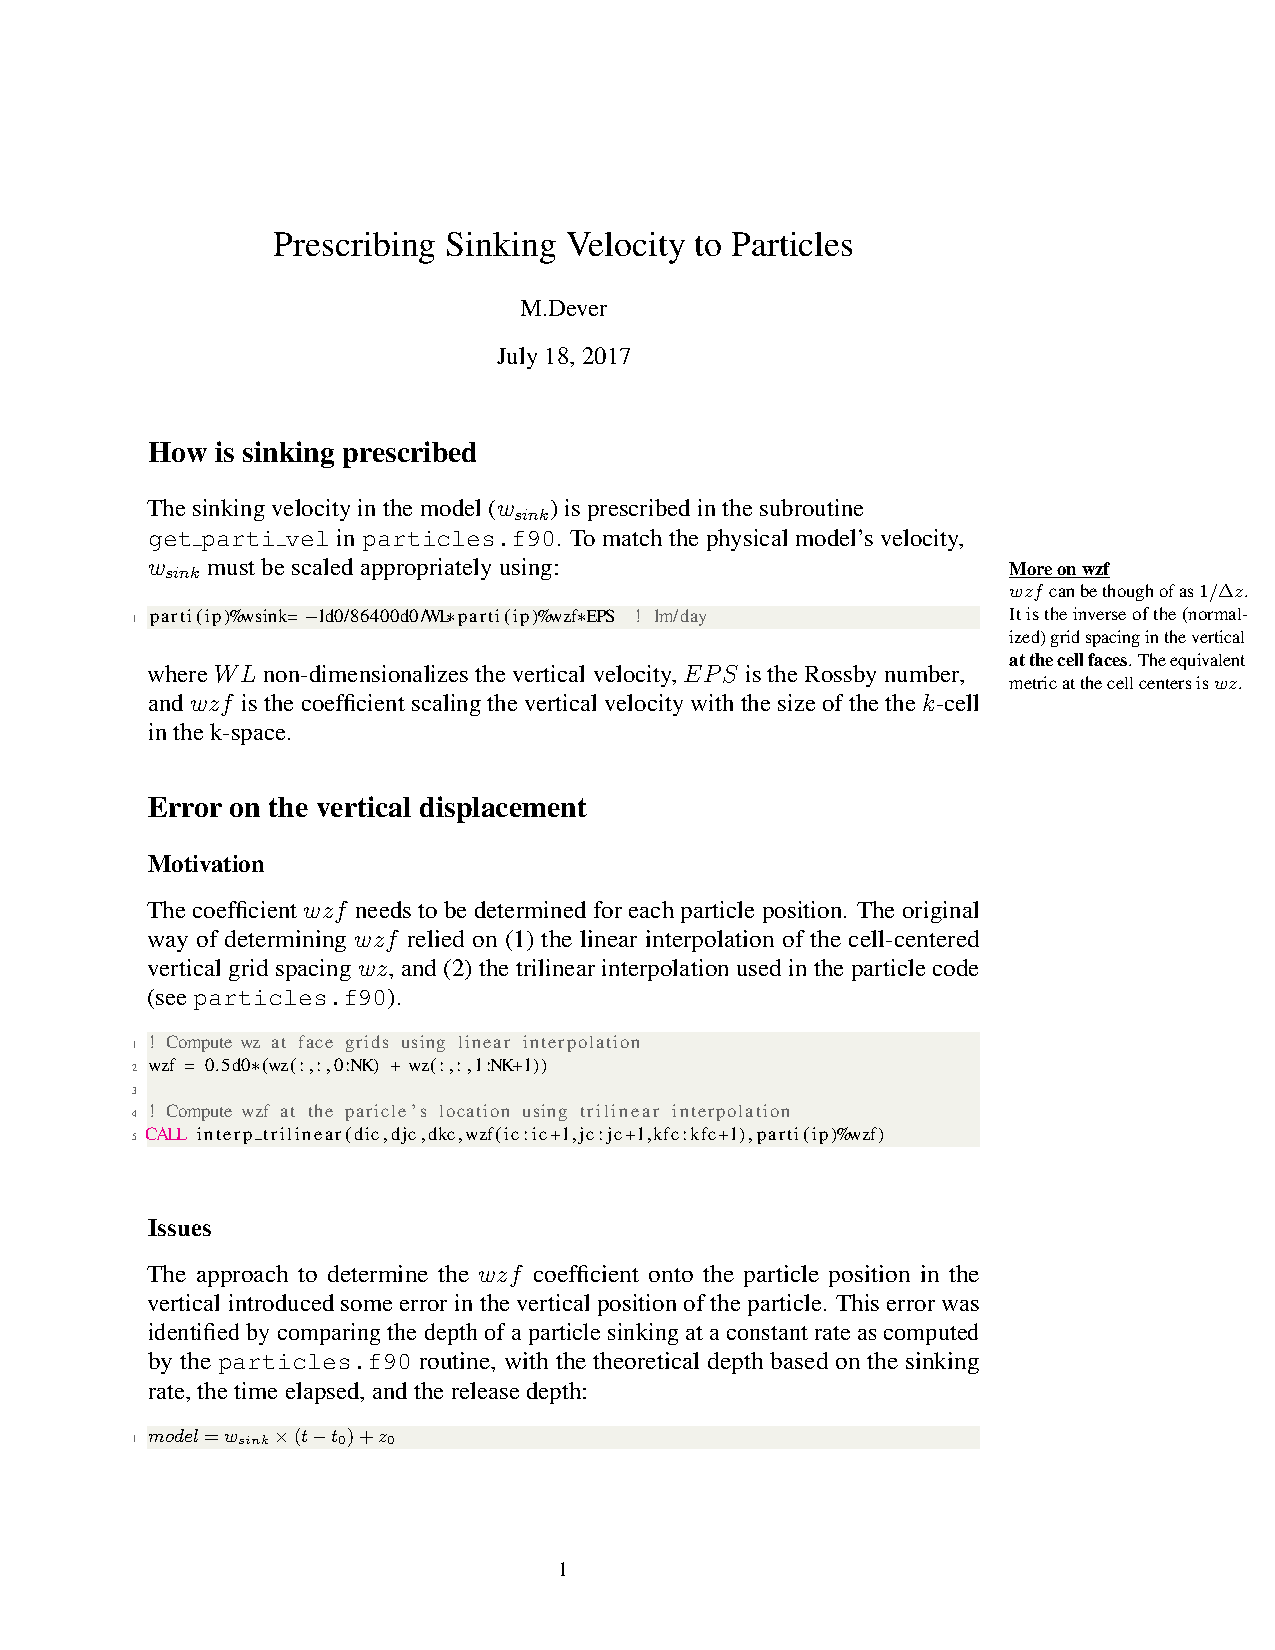
\includepdf[pages={1-3}]{appendices/notes_on_sinking_velocity.pdf}

\section{Appendix B - particle\_open\_bin.m}
\label{app: particle_open_bin}
\begin{lstlisting}[language=matlab]
clear

% ** This code imports the particle-tracking data directly from bin output
% files. 
% ** The file path has to be specified.
% ** output is a 3D matrix where the 1st dimension is the particle number,
% the 2nd dimension is the model time, and the 3rd diemnsion is the
% recorded variables.

%%%%%%%%%%%%%%%%%%%%%%%%
% WARNING
%%%%%%%%%%%%%%%%%%%%%%%%
% This routine SHOULD NOT BE USED FOR LARGE FILES otherwise MATLAB matrices
% will become too large and will crash MATLAB.
%%%%%%%%%%%%%%%%%%%%%%%%

%%
%%%%%%%%%%%%%%%%%%%%%%%%
% PARAMETERS
%%%%%%%%%%%%%%%%%%%%%%%%

% number of files to import into matlab
number_of_files = 1;
% filepath
path = 'specify the path for the output files here';
% Number of variables recorded (see particles.f90)
number_of_variables = 20;

%%%%%%%%%%%%%%%%%%%%%%%%
% CORE CODE
%%%%%%%%%%%%%%%%%%%%%%%%

% Loops through the nummber of files to open
for filenum = 1:number_of_files

% Create fullpath
filename = ['op.parti-',num2str(filenum,'%03.f'),'.bin'];
fullpath = [path,'/',filename];

% Display the file being extracted
disp(filename);

% Open the file
fileID = fopen(fullpath);

% Extract the data (refer to particles.f90 to confirm that number) 
A = fread(fileID,[number_of_variables Inf],'double');
A = A';

% Finds the number of particle per file using the ID numbers
if filenum == 1
partnum = max(A(:,1));
end

% write a matrix of dimensions:
% # of particles x timestep x recorded variables
for Np = (filenum-1)*partnum+1:(filenum-1)*partnum+partnum
ind = find(A(:,1) == Np);
data(Np,:,:) = A(ind,:);
end; clear Np ind

fclose(fileID);
clear A fileID filename path fullpath ans

end; clear filenum partnum
\end{lstlisting}
\pagebreak

\section{Appendix C - particle\_bin2csv}
\label{app: particle_bin2csv}
\begin{lstlisting}[language=matlab]
clear

% This code converts the binary file ouput from the model into CSV files.
% This can be useful to open in other programs (e.g., import in a SQL
% database)

%%
%%%%%%%%%%%%%%%%%%%%%%%%
% PARAMETERS
%%%%%%%%%%%%%%%%%%%%%%%%

% number of files to import into matlab
number_of_files = 1;
% filepath of files to import
pathin = 'specify the path of the files to import here';
% Number of variables recorded (see particles.f90)
number_of_variables = 20;
% filepath of the csv-file to be written
pathout = 'specify the path where you would like to write the csv-files';

%%%%%%%%%%%%%%%%%%%%%%%%
% CORE CODE
%%%%%%%%%%%%%%%%%%%%%%%%

% Loops through the number of files to open
for filenum = 1:number_of_files
    
    % Create fullpath
    filename = ['op.parti-',num2str(filenum,'%03.f'),'.bin'];
    fullpath = [pathin,'/',filename];
    
    % Display the file being extracted
    disp(['Converting ',filename,' into a CSV file ...']);
    
    % Open the file
    fileID = fopen(fullpath);
    
    % Extract the data (refer to particles.f90 to confirm that number)
    A = fread(fileID,[number_of_variables Inf],'double');
    A = A';
    
    % Remove all the zeros recorded
    ind = find(A(:,1)==0);
    if isempty(ind)~=1
        warning(['Missing ',num2str(length(ind)),' records...!'])
        A(ind,:) = [];
    end; clear ind
    
    
    % Re-write the file as CSV.
    csvwrite([pathout,'/op.parti-',num2str(filenum,'%03.f'),'.csv'],A)
    
    fclose(fileID);
    clear A partnum fileID filename path fullpath
    
end; clear filenum
\end{lstlisting}

%Print the glossary
\pagebreak
\glsaddall				% Include all glossary entries
\glossarystyle{listhypergroup}	% Define style for glossary
\renewcommand*{\arraystretch}{0.3}% default is 1
\printglossaries

\end{document}
